\section{Specific Model Of Bovine Viral Diarrhea}
\label{chap:bvdModel}
The basic SIR-Model as it is discussed in chapter \ref{chap:generalModeling} is unfortunately not sufficient to describe a complex illness like BVD. This section therefore tries to give a brief introduction to the disease and how it can be modeled.

Disclaimer: Since this is a thesis that is supposed to focus on the theoretical and mathematical description and interpretation of the phenomena observed around BVD (and the Virus BVDV), the introduction to the biological phenomena will be rather short. For this purpose the author relies on \citep{LIN03}, which is a paper that has been cited a lot and which has been published $14\,\text{years}$ earlier to this thesis, which is why the author with his limited knowledge about the field has the humble opinion that it is a very reliable source.

\subsection{BVD Basics}\label{chap:bvdBasics}
Bovine Viral Diarrhea is a virus infection that leads to various symptoms depending on the status of the cow. Most of the effects which will be neglected in the modeling of the disease will also be neglected in this explanation.

\paragraph{Non Pregnant Cows} If a bovine get's infected while not being pregnant, the numbers of white blood cells and thrombocytes decrease. According to \citep{LIN03} this can even lead to a lessened semen quality in infected bulls where the virus may even persist in the testicles. Furthermore the virus can be detected $4 \text{ to } 10\,\text{days}$ after infection in most secretes and \glqq clinical symptoms such as fever, post infection, inappetence and mucosal lesions\grqq. The symptom that gave this disease it's name, diarrhea, as well as coughing are mostly seen in calves, but it's not entirely clear if this might be due to a secondary infection that is caused by the immune suppressive effect of the loss of white blood cells and thrombocytes.
A recovered cow with a normally working immune system will be immune to BVDV for the rest of it's life and it's calves will also be protected by the maternal antibodies in the cow's milk for the first $4-6\, \text{months}$ of their lives. If calves get vaccinated while being protected by maternal antibodies, the vaccination won't protect them from the disease. However the majority of farmers mixes their colostrum \citep{personalCom}. This can lead to a bigger group of immune calves, but it could possibly dilute the antibody levels below the threshold where it actually creates an immune response.

\paragraph{Pregnant Cows}
For the mother the virus will have little implications, but the unborn calve can suffer a various number of complications. The mother can become infertile, while the calve can die, have malformations, be retarded, weak or stillborn, but most importantly some calves could become persistently infected (PIs). These calves will be infectious during their whole life time and produce high amounts of the virus. Their body does not detect the virus as harmful and therefore doesn't not build up antibodies \citep{personalCom}. Calves of PIs are always PIs too. PIs have a much shorter life span, especially because they can suffer secondary illnesses such as mucosal disease which triggers diarrhea and can be survived by chronic cases for up to $18\,\text{months}$.

\subsection{Compartmental Model}
The alert reader may have noticed that BVD as it's discussed in chapter \ref{chap:bvdBasics} could be described with a SIR-Model with slight modifications. 
\begin{figure}[htbp]
\centering
\noindent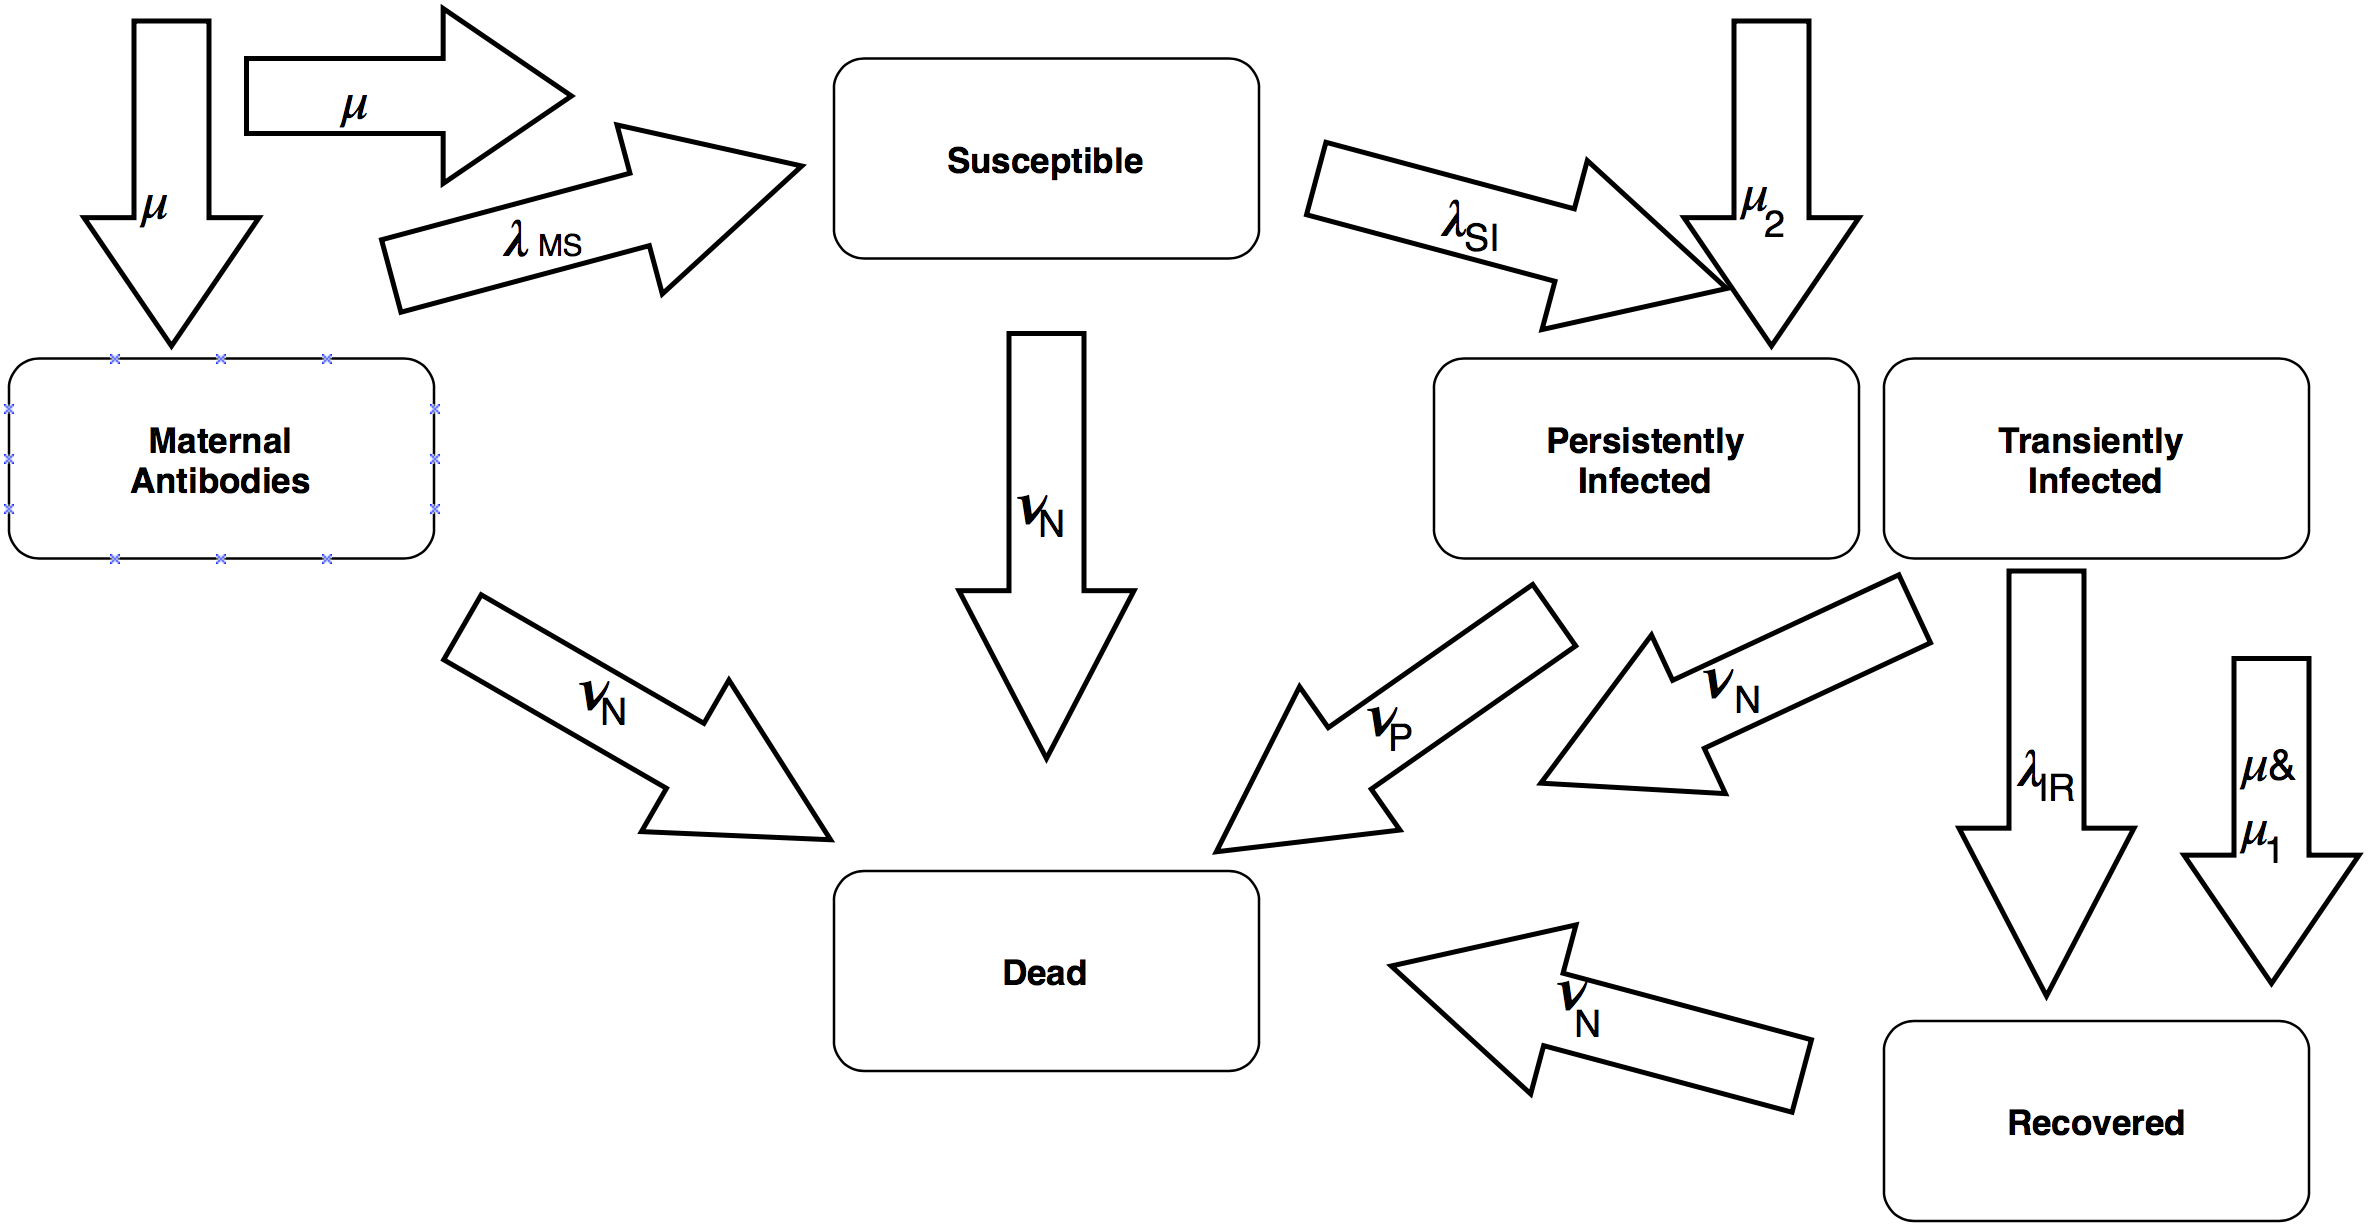
\includegraphics[width=\linewidth,height=\textheight,
keepaspectratio]{bvdDia.png} \caption[]{This plot shows }
\label{fig:bvdDia}
\end{figure}
In addition to the model we add two new groups: the group of calves protected by maternal antibodies in their milk, the MAs, the group of persistently infected cows, the PIs, and in order to make it easier to differentiate between the two groups of infected, the group normally marked as I will be called TI\footnote{In order to improve the readability of of all equations PIs will be marked as $P$, MAs as $M$ and TIs as $I$.}.
 With a death rate of non PIs $\nu_\text{N}$, a death rate of PIs $\nu_\text{P}$, a general birth rate $\mu$ and birth rates for recovered $\mu_1$ and PIs $\mu_2$ after an infected met a susceptible at the right point in time we get:

\begin{eqnarray}
\dot{M}  =& \mu R-\lambda_\text{MS} M -\nu_\text{N} M & \\
\dot{S}  =& \lambda_\text{MS} M - \lambda_\text{SI}SI-\lambda_\text{SP} SP &-\nu_\text{N} S + \mu S \\
\dot{I}  =& \beta_\text{SI}SI+\beta_\text{SP} SP - \lambda_\text{IR} I &- \nu_\text{N} I \label{eq:idotbvd} \\
\dot{R}  =& \lambda_\text{IR}I - \nu_\text{N} R +\mu_1S(t-\tau_1)I(t-\tau_1) &+\mu_1S(t-\tau_1)P(t-\tau_1) \\ 
\dot{P}  =&  \mu P -\nu_\text{P}P + \mu_2S(t-\tau_2)I(t-\tau_2) &+ \mu_2S(t-\tau_2)P(t-\tau_2)
\end{eqnarray}
following \citep{BAS16} with the infection probabilities when a PI or a TI meet a susceptible $\beta_\text{PI}$ and $\beta_\text{TI}$. The time delays $(t-\tau_1)$ and $(t-\tau_2)$ are visualized in \ref{fig:infectionTimeScale} 
\footnote{This thing is super wrong according to "BVD Programm.doc"}. Equation \ref{eq:idotbvd} can be rewritten like:
\begin{eqnarray}
\dot{I}  =& \lambda_\text{SIges}S - \lambda_\text{IR}&I - \nu_\text{N} I, \text{ with} \\
\lambda_\text{SI} =& \beta_\text{SI} I+ \beta_\text{PI} P.& \label{eq:vie04start}
\end{eqnarray}

\begin{figure}[htbp]
\centering
\noindent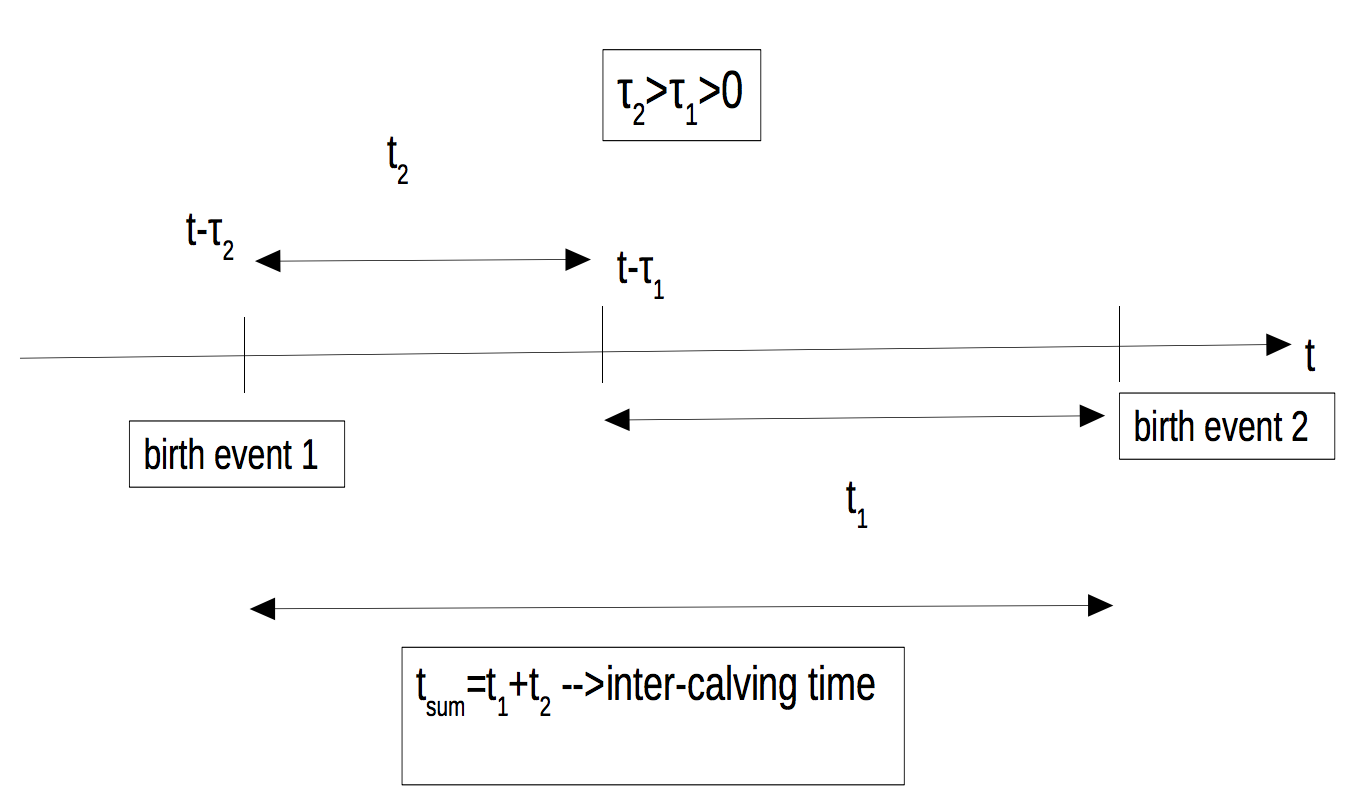
\includegraphics[width=\linewidth,height=\textheight,
keepaspectratio]{infectionTimeScale.png} \caption[]{This plot shows }
\label{fig:infectionTimeScale}
\end{figure}
